\section{Week 3 - Linear Response Theory continued}
\paragraph{Agenda:}
\begin{itemize}
    \item Optical transitions in Hartree Fock 
    \item Density Functional Theory
    \item Static Screening in metals
    \begin{itemize}
        \item Thomas Fermi, $\omega = 0$
        \item Lindhard function $\{q,r\}$-dependence
    \end{itemize}
    \item Dynamical screening
    \begin{itemize}
        \item Drude model
        \item Lindhard model
        \item Long wavelength limit, a.k.a. optimal limit.
        \item $\{\omega,t\}$-dependence
    \end{itemize}
\end{itemize}
Since we are working with the homogeneous electron gas (EG), we have complete translational invariance and hence $\chi\qty(r,r',\omega) = \chi \qty(r - r',\omega)$ and the FT becomes $\chi\qty(q,q',\omega) = \chi\qty(q,\omega)\delta\qty(q-q') $ \\ 
\paragraph{Note that:}
$E_{\mathrm{LUMO}} = E_{\mathrm{AF}}$, where AF denotes the electron affinity.\\
$E_{\mathrm{HOMO}} = E_{\mathrm{IP}}$ where IP denotes the ionisation potential. \\
\paragraph{Quote of the day:}
\emph{"You should never do anything that smells a bit like Hartree Fock for metals"} - Kristian Sommer Thygesen (2018). This is due to an infinite derivative in the dispersion relation at $k=k_F$, which is due to the way that the exchange is introduced as a product rather than the integral over a product.\\
We construct the effective potential s.t. the non-interacting system has the same ground state density as the interacting system.

\subsection{DFT}
We want to evaluate the ground state energy:
\paragraph{Hohenberg-Kohn Theorem} There exists a 1-1 correspondence between the ground state electron density and the external potential.\\
\emph{Consequence:} The ground state energy is a functional of the ground state density.

\begin{figure}[h!]
    \centering
    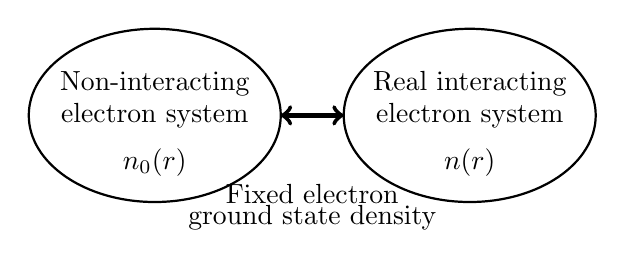
\begin{tikzpicture}
        \draw[thick] (-2,0) ellipse (1.6cm and 1.1cm);
        \draw[thick] (2,0) ellipse (1.6cm and 1.1cm);
        \draw[ultra thick,<->] (-0.4,0)--(0.4,0);
        \node[] at (-2,0.4) {Non-interacting};
        \node[] at (-2,0) {electron system};
        \node[] at (-2,-0.6) {$n_0(\vb{r})$};
        \node[] at (2,0.4) {Real interacting};
        \node[] at (2,0) {electron system};
        \node[] at (2,-0.6) {$n(\vb{r})$};
        \node[] at (0,-1) {Fixed electron};
        \node[] at (0,-1.3) {ground state density};
    \end{tikzpicture}
    \caption{Kohn-Sham ansatz}
    \label{fig:dft_ks_ansatz}
\end{figure}
This paper will in terms of \emph{Density Functinal Theory} (DFT) mainly focus on the self-consistent Kohn-Sham (KS) approach which was used in the computational part of the project. One can say that the self-consistent single-particle equations proposed by Hartree back in 1928 set the frame for the Kohn-Sham equations. \\ Back in 1964, Pierre Hohenberg and Walter Kohn took the first huge step in the development of modern DFT by proving that knowing the electron density in the ground state is enough for one to describe the whole system. In the winter of 1964, Kohn and Lu Jeu Sham then sat together and combined the Hohenberg-Kohn variational principle which in theory was exact for the ground-state together with the Hartree equations to form an, in principle, exact Hartree-like formulation, the Kohn-Sham equations.
\cite{KohnNobelLecture} \\
The Kohn-Sham approach is based on the assumption that one can find a ground state density for a fictitious system of non-interacting particles corresponding to the exact ground state density for the real interacting electron system as illustrated in figure \ref{fig:dft_ks_ansatz}. This non-interacting reference system is described by an effective potential and the usual kinetic term,
\begin{equation} 
\label{eq:reference_system_KS}
\hat{H}_R = - \dfrac{\hbar^2}{2m} \nabla^2 + v_R \qty(\vb{r})
\end{equation}
The difficult part in the Kohn-Sham ansatz is then to find such an effective potential for a given system which satisfies that the ground-state density can be written as a probability distribution over the single particle eigenfunctions; mathematically speaking,
\begin{equation}
\hat{H}_R = \varepsilon_i \phi_i \qty(\vb{r}) \qquad \qquad \sum_{i=1}^N \abs{\phi_i \qty(\vb{r})}^2 = n_0 \qty(\vb{r})
\end{equation}
Walter Kohn and Lu Jeu Sham got the idea to rewrite the Hohenberg-Kohn energy functional into large knows terms and put the unknowns into a new term, the so-called \emph{exchange-correlation functional}, $E_{xc}[n]$,
\begin{equation}\label{eq:kohn_sham_ef}
\begin{split}
    E[n] &= T[n] + U_{ee} [n] + \int v_{ion} \qty(\vb{r}) n \qty(\vb{r}) \difd \vb{r} \\
    &=T_s\qty[n] + U_{ee} \qty[n] + \int v_{ion} \qty(\vb{r}) n \qty(\vb{r}) \mathrm{d}\vb{r} + E_{xc} \qty[n] \\
    &= \underbrace{T_s \qty[n]}_\text{Non-interacting} + \underbrace{\dfrac{1}{2} \int \int \dfrac{n\qty(\vb{r'}) n\qty(\vb{r})}{\qty|\vb{r}-\vb{r'}|} \mathrm{d}\vb{r'} \, \mathrm{d}\vb{r}}_\text{Hartree} + \int v_{ion} \qty(\vb{r}) n \qty(\vb{r}) \mathrm{d}\vb{r} + \underbrace{ E_{xc} \qty[n]}_\text{Exchange-Correlation}
\end{split}
\end{equation}
In \eqref{eq:kohn_sham_ef}, the interacting kinetic energy term is split up to a non-interactive term plus a correlation term which is put into $E_{xc}[n]$. This means that this this fictitious wave function constructed by the eigenfunctions is treated as a single Slater determinant even though the real wave function can not. If this can be done under the constraint that the electron density remains the same, one can in principle obtain the right ground state energy even though the individual terms in the expression might be off energy-wise. However, the exact ground state energy can only be evaluated if the right exchange-correlation functional is used. And unfortunately, it is non an easy tasks to construct these functionals. The $U_{ee}[n]$ term in \ref{eq:kohn_sham_ef} is split up into the term one may know from classical Hartree theory and an unknown exchange-correlation term put into $E_{xc}[n]$ as well. \\

By using Euler's equation and Lagrange multipliers to assure particle conservation on \eqref{eq:kohn_sham_ef} and \eqref{eq:reference_system_KS}, one can combine the two Euler-Lagrange equations to obtain the effective potential, $v_R \qty(\vb{r})$:
\begin{equation}\label{eq:CombiningEuler}
\begin{split} 
v_R \qty(\vb{r}) &= \int \dfrac{n \qty(\vb{r'})}{\abs{\vb{r}-\vb{r'}}} \difd\vb{r'} + v_{ion} \qty(\vb{r}) + \dfrac{\delta E_{xc} \qty[n]}{\delta n } \\
&= v_H \qty(\vb{r}) + v_{ion} \qty(\vb{r}) + v_{xc} \qty(\vb{r})
\end{split}
\end{equation}
With this effective potential, one can try to solve single-particle Schrödinger's equations for the reference system. This is known as the Kohn-Sham self-consistency problem and in this way, Kohn and Sham created a density functional based formulation of Hartree's  work.

\subsection{The Kohn-Sham self-consistency equations}
\begin{figure}[h!]
    \centering
    \begin{tikzpicture}
        \filldraw[fill=blue!20!white,dashed, thick, rounded corners=15pt] (-1.5,3) rectangle (1.5,4);
        \filldraw[fill=blue!20!white,ultra thick, rounded corners=15pt ] (-3.5,0.5) rectangle (3.5,2);
        \filldraw[fill=blue!20!white,ultra thick, rounded corners=15pt] (-3.5,-2) rectangle (3.5,-0.5);
        \filldraw[fill=blue!20!white,ultra thick, rounded corners=15pt] (-3.5,-4.5) rectangle (3.5,-3);
        \draw[ultra thick,->, rounded corners=15pt] (3.5,-3.75)--(4.5,-3.75)--(4.5,1.25)--(3.5,1.25);
        \draw[->, ultra thick] (0,3)--(0,2);
        \draw[->, ultra thick] (0,0.5)--(0,-0.5);
        \draw[->, ultra thick] (0,-2)--(0,-3);
        \node[] at (0,3.5) {Initial guess $n(\vb{r})$};
        \node[] at (0,1.25) {$v_R \qty(\vb{r}) = \int \dfrac{n \qty(\vb{r'})}{\abs{\vb{r}-\vb{r'}}} \difd\vb{r'} + v_{ion} \qty(\vb{r}) + \dfrac{\delta E_{xc} \qty[n]}{\delta n }$};
        
        \node[] at (0, -1.25) {$\qty(- \dfrac{\hbar^2}{2m} \nabla^2 + v_R \qty(\vb{r}))\phi_i\qty(\vb{r})=\varepsilon_i\phi_i\qty(\vb{r})$};
        \node[] at (0,-3.75) { $n\qty(\vb{r})= \sum_{i=1}^N \abs{\phi_i \qty(\vb{r})}^2$ };
        \node[anchor=south east] at (0,2) {Effective potential};
        \node[anchor=south east] at (0,-0.5) {Solve single-particle equation};
        \node[anchor=south east] at (0,-3) {Calculate new density};
    \end{tikzpicture}
    \caption{Hartree-like self-consistency problem}
    \label{fig:self_consistency_KS}
\end{figure}
This self-consistency problem looks a lot like Hartree's. The difference is in the inclusion of an exchange-correlation term. \\ 
As shown in figure \ref{fig:self_consistency_KS}, the procedure starts with a guess for the ground state density to which the effective potential can be constructed and Schrödinger's time-independent eigenvalue problem can be solved. These eigenfunctions then corresponds to a new density which is then put into the effective potential. The iterations continue until the ground state density is reached corresponding to the lowest energy. \\
In the Kohn-Sham approach, the ground state energy can be found to be given as \eqref{ground_state_energy}
\begin{equation}\label{ground_state_energy}
    E = \sum _j \varepsilon_j + E_{xc} \qty[n(\vb{r})]- \int v_{xc} (\vb{r}) n (\vb{r}) \dd v - \dfrac{1}{2} \int \dfrac{n(\vb{r}) n(\vb{r'})}{\abs{r-r'}}
\end{equation}

Having said that, the exchange-correlation functional, $E_{xc}[n]$, remains unknown and has to be approximated. Nowadays, there are huge databases with exchange-correlation functional and one may choose different functionals depending on what atomic property one is seeking to calculate. The choice of functional also depends on how accurate the calculation needs to be due to the time consumption being highly functional dependent. Jacob's ladder is often used in terms of DFT; the more accurate the simulation needs to be, the more expensive it is in terms of time/computation. \\
In this project, mainly a generalized gradient approximation (GGA) functional by the name PBE after Perdew,Burke and Ernzerhof has been used. The general stucture of a GGA functional is,
\begin{equation}
    E_{xc}[n]= \int n \qty(\vb{r}) \varepsilon_{xc} \comm{n\qty(\vb{r})}{ \nabla n \qty(\vb{r})} \dd \vb{r}
\end{equation}
where $\varepsilon_{xc}$ is the exchange-correlation hole. The GGA functional, PBE, was mainly chosen because of the relatively low computational costs and band structure preserving properties.

\subsection{Static screening, $\omega = 0$}
\paragraph{Thomas-Fermi model} (
\textbf{PROVE} that the induced potential from a plane-wave external potential must also be a plane-wave with the same wave vector.)\\
Relating the external and total potential:
\begin{equation}
\begin{split}
    U_{ext}(r) &= A_{ext}(q) \mathrm{e}^{iqr} + c.c \\
    U_{tot}(r) &= A_{tot}(q) \mathrm{e}^{iqr} + c.c
\end{split}
\end{equation}
where the induced electron density due to the external potential is, $n_{ind} = - \rho\qty(E_F) U_{tot}(r)$.

\paragraph{Remember the following FT:}
\begin{equation}
    \dfrac{1}{r}= \int  \dfrac{1}{q^2} \mathrm{e}^{i \vb{q}\cdot \vb{r}} d\vb{q}
\end{equation}
\paragraph{NB.} Potentials are exponentially screened in TF theory. In metals, $k_F^{-1} \approx a_0 \approx 0.5$Å. 

\subsection{Dynamical screening, $q =  0$}

